% ------------------------------------------------------------------------
% AMS-LaTeX Paper ********************************************************
% ------------------------------------------------------------------------
% Submitted:      Dec 15 2003
% Final Version:  
% Accepted:       
% ------------------------------------------------------------------------
% This is a journal top-matter template file for use with AMS-LaTeX.
%%%%%%%%%%%%%%%%%%%%%%%%%%%%%%%%%%%%%%%%%%%%%%%%%%%%%%%%%%%%%%%%%%%%%%%%%%

% TODO(mike): locating a closure at a name: how to translate a closure into a process that gets stuck into the cell



%\documentclass{tran-l}
%\documentclass[twocolumn]{amsart}
%\documentclass[]{amsart}
%\documentclass[]{sig-alternate}
\documentclass[]{acm_proc_article-sp}
%\documentclass[]{llncs}

%\documentclass[]{prentcsmacro}

%\usepackage[active]{srcltx} % SRC Specials for DVI Searching
\usepackage{url}

% From Allen's stable.
\usepackage{bigpage}
\usepackage{bcprules}
%\usepackage{code}
\usepackage{mathpartir}
\usepackage{listings}
\usepackage{mathtools}
%\usepackage[fleqn]{amsmath}
\usepackage{amsfonts}
\usepackage{latexsym}
\usepackage{amssymb}
\usepackage{caption}
\usepackage{tikz}
%\usepackage{multicol}

\newcommand{\maps}{\colon}
% Double brackets
\newcommand{\ldb}{[\![}
\newcommand{\rdb}{]\!]}
\newcommand{\ldrb}{(\!(}
\newcommand{\rdrb}{)\!)}
\newcommand{\lliftb}{\langle\!|}
\newcommand{\rliftb}{|\!\rangle}
% \newcommand{\lpquote}{\langle}
% \newcommand{\rpquote}{\rangle}
% \newcommand{\lpquote}{\lceil}
% \newcommand{\rpquote}{\rceil}
\newcommand{\lpquote}{\ulcorner}
\newcommand{\rpquote}{\urcorner}
\newcommand{\newkw}{\nu}

% SYNTAX
\newcommand{\id}[1]{\texttt{#1}}
\newcommand{\none}{\emptyset}
\newcommand{\eps}{\epsilon}
\newcommand{\set}[1]{\{#1\}}
\newcommand{\rep}[2]{\id{\{$#1$,$#2$\}}}
\newcommand{\elt}[2]{\id{$#1$[$#2$]}}
\newcommand{\infinity}{$\infty$}

\newcommand{\pzero}{\mathbin{0}}
\newcommand{\seq}{\mathbin{\id{,}}}
\newcommand{\all}{\mathbin{\id{\&}}}
\newcommand{\choice}{\mathbin{\id{|}}}
\newcommand{\altern}{\mathbin{\id{+}}}
\newcommand{\juxtap}{\mathbin{\id{|}}}
%\newcommand{\concat}{\mathbin{.}}
\newcommand{\concat}{\Rightarrow}
\newcommand{\punify}{\mathbin{\id{:=:}}}
\newcommand{\fuse}{\mathbin{\id{=}}}
\newcommand{\scong}{\mathbin{\equiv}}
\newcommand{\nameeq}{\mathbin{\equiv_N}}
\newcommand{\alphaeq}{\mathbin{\equiv_{\alpha}}}
\newcommand{\names}[1]{\mathbin{\mathcal{N}(#1)}}
\newcommand{\freenames}[1]{\mathbin{\mathcal{FN}(#1)}}
\newcommand{\boundnames}[1]{\mathbin{\mathcal{BN}(#1)}}
%\newcommand{\lift}[2]{\texttt{lift} \; #1 \concat #2}
\newcommand{\binpar}[2]{#1 \juxtap #2}
\newcommand{\outputp}[2]{#1 ! ( * #2 )}
\newcommand{\prefix}[3]{#1 ? ( #2 ) \concat #3}
\newcommand{\lift}[2]{#1 ! ( #2 )}
%\newcommand{\quotep}[1]{\lpquote #1 \rpquote}
\newcommand{\quotep}[1]{@#1}
\newcommand{\dropn}[1]{*#1}

\newcommand{\newp}[2]{\id{(}\newkw \; #1 \id{)} #2}
\newcommand{\bangp}[1]{\int #1}
\newcommand{\xbangp}[2]{\int_{#2} #1}
\newcommand{\bangxp}[2]{\int^{#2} #1}

\newcommand{\substp}[2]{\id{\{} \quotep{#1} / \quotep{#2} \id{\}}}
\newcommand{\substn}[2]{\id{\{} #1 / #2 \id{\}}}

\newcommand{\psubstp}[2]{\widehat{\substp{#1}{#2}}}
\newcommand{\psubstn}[2]{\widehat{\substn{#1}{#2}}}

\newcommand{\applyp}[2]{#1 \langle #2 \rangle}
\newcommand{\absp}[2]{\id{(} #1 \id{)} #2}

\newcommand{\transitions}[3]{\mathbin{#1 \stackrel{#2}{\longrightarrow} #3}}
\newcommand{\meaningof}[1]{\ldb #1 \rdb}
\newcommand{\pmeaningof}[1]{\ldb #1 \rdb}
\newcommand{\nmeaningof}[1]{\ldrb #1 \rdrb}

\newcommand{\Proc}{\mathbin{Proc}}
\newcommand{\QProc}{\quotep{\mathbin{Proc}}}

\newcommand{\entailm}{\mathbin{\vdash_{\mathfrak m}}} %matching
\newcommand{\entailp}{\mathbin{\vdash_{\mathfrak p}}} %behavioral
\newcommand{\entailv}{\mathbin{\vdash_{\mathfrak v}}} %validation
\newcommand{\congd}{\mathbin{\equiv_{\mathfrak d}}}
\newcommand{\congs}{\mathbin{\equiv_{\mathfrak s}}}
\newcommand{\congp}{\mathbin{\equiv_{\mathfrak p}}}
%\newcommand{\defneqls}{:\!=}
\newcommand{\defneqls}{\coloneqq}
%\newcommand{\logequiv}{\mathbin{\leftrightarrow}}

\newcommand{\barb}[2]{\mathbin{#1 \downarrow_{#2}}}
\newcommand{\dbarb}[2]{\mathbin{#1 \Downarrow_{#2}}}

% From pi-duce paper
\newcommand{\red}{\rightarrow}
\newcommand{\wred}{\Rightarrow}
\newcommand{\redhat}{\hat{\longrightarrow}}
\newcommand{\lred}[1]{\stackrel{#1}{\longrightarrow}} %transitions
\newcommand{\wlred}[1]{\stackrel{#1}{\Longrightarrow}}

\newcommand{\opm}[2]{\overline{#1} [ #2 ]} % monadic
\newcommand{\ipm}[2]{{#1} ( #2 )} 
\newcommand{\ipmv}[2]{{#1} ( #2 )} % monadic
\newcommand{\parop}{\;|\;}		% parallel operator
\newcommand{\patmatch}[3]{#2 \in #3 \Rightarrow #1}
\newcommand{\sdot}{\, . \,}		% Space around '.'
\newcommand{\bang}{!\,}
%\newcommand{\fuse}[1]{\langle #1 \rangle}		
\newcommand{\fusion}[2]{#1 = #2} % fusion prefix/action
\newcommand{\rec}[2]{\mbox{\textsf{rec}} \, #1. \, #2}
\newcommand{\match}[2]{\mbox{\textsf{match}} \; #1 \; \mbox{\textsf{with}} \; #2}
\newcommand{\sep}{:}
\newcommand{\val}[2]{\mbox{\textsf{val}} \; #1 \; \mbox{\textsf{as}} \; #2}

\newcommand{\rel}[1]{\;{\mathcal #1}\;} %relation
\newcommand{\bisim}{\stackrel{.}{\sim}_b} %bisimilar
\newcommand{\wb}{\approx_b} %weak bisimilar
\newcommand{\bbisim}{\stackrel{\centerdot}{\sim}} %barbed bisimilar
\newcommand{\wbbisim}{\stackrel{\centerdot}{\approx}} %weak barbed bisimilar
\newcommand{\bxless}{\lesssim}	%expansion less (amssymb required)
\newcommand{\bxgtr}{\gtrsim}	%expansion greater (amssymb required)
\newcommand{\beq}{\sim}		%barbed congruent
\newcommand{\fwbeq}{\stackrel{\circ}{\approx}}	%weak barbed congruent
\newcommand{\wbeq}{\approx}	%weak barbed congruent
\newcommand{\sheq}{\simeq}	%symbolic hypereq
\newcommand{\wbc}{\approx_{cb}}

% End piduce contribution

% rho logic

\newcommand{\ptrue}{\mathbin{true}}
\newcommand{\psatisfies}[2]{#1 \models #2}
\newcommand{\pdropf}[1]{\rpquote #1 \lpquote}
\newcommand{\pquotep}[1]{\lpquote #1 \rpquote}
\newcommand{\plift}[2]{#1 ! ( #2 )}
\newcommand{\pprefix}[3]{\langle #1 ? #2 \rangle #3}
\newcommand{\pgfp}[2]{\textsf{rec} \; #1 \mathbin{.} #2}
\newcommand{\pquant}[3]{\forall #1 \mathbin{:} #2 \mathbin{.} #3}
\newcommand{\pquantuntyped}[2]{\forall #1 \mathbin{.} #2}
\newcommand{\riff}{\Leftrightarrow}

\newcommand{\PFormula}{\mathbin{PForm}}
\newcommand{\QFormula}{\mathbin{QForm}}
\newcommand{\PropVar}{\mathbin{\mathcal{V}}}

\newcommand{\typedby}{\mathbin{\:\colon}}
\newcommand{\mixedgroup}[1]{\id{mixed($#1$)}}
\newcommand{\cast}[2]{\id{CAST AS} \; #1 \; (#2)}
\newcommand{\bslsh}{\mathbin{\id{\\}}}
\newcommand{\bslshslsh}{\mathbin{\id{\\\\}}}
\newcommand{\fslsh}{\mathbin{\id{/}}}
\newcommand{\fslshslsh}{\mathbin{\id{//}}}
\newcommand{\bb}[1]{\mbox{#1}}
\newcommand{\bc}{\mathbin{\mathbf{::=}}}
\newcommand{\bm}{\mathbin{\mathbf\mid}}
\newcommand{\be}{\mathbin{=}}
\newcommand{\bd}{\mathbin{\buildrel {\rm \scriptscriptstyle def} \over \be}}
\newcommand{\ctcategory}[1]{\mbox{\bf #1}}

%GRAMMAR
\newlength{\ltext}
\newlength{\lmath}
\newlength{\cmath}
\newlength{\rmath}
\newlength{\rtext}

\settowidth{\ltext}{complex type name}
\settowidth{\lmath}{$xxx$}
\settowidth{\cmath}{$::=$}
\settowidth{\rmath}{\id{attributeGroup}}
\settowidth{\rtext}{repetition of $g$ between $m$ and $n$ times}

\newenvironment{grammar}{
  \[
  \begin{array}{l@{\quad}rcl@{\quad}l}
  \hspace{\ltext} & \hspace{\lmath} & \hspace{\cmath} & \hspace{\rmath} & \hspace{\rtext} \\
}{
  \end{array}\]
}

% Over-full v-boxes on even pages are due to the \v{c} in author's name
\vfuzz2pt % Don't report over-full v-boxes if over-edge is small

% THEOREM Environments ---------------------------------------------------
 \newtheorem{thm}{Theorem}[subsection]
 \newtheorem{cor}[thm]{Corollary}
 \newtheorem{lem}[thm]{Lemma}
 \newtheorem{prop}[thm]{Proposition}
% \theoremstyle{definition}
 \newtheorem{defn}[thm]{Definition}
% \theoremstyle{remark}
 \newtheorem{rem}[thm]{Remark}
 \newtheorem{example}[thm]{Example}
 \numberwithin{equation}{subsection}
% MATH -------------------------------------------------------------------
 \DeclareMathOperator{\RE}{Re}
 \DeclareMathOperator{\IM}{Im}
 \DeclareMathOperator{\ess}{ess}
 \newcommand{\veps}{\varepsilon}
 \newcommand{\To}{\longrightarrow}
 \newcommand{\h}{\mathcal{H}}
 \newcommand{\s}{\mathcal{S}}
 \newcommand{\A}{\mathcal{A}}
 \newcommand{\J}{\mathcal{J}}
 \newcommand{\M}{\mathcal{M}}
 \newcommand{\W}{\mathcal{W}}
 \newcommand{\X}{\mathcal{X}}
 \newcommand{\BOP}{\mathbf{B}}
 \newcommand{\BH}{\mathbf{B}(\mathcal{H})}
 \newcommand{\KH}{\mathcal{K}(\mathcal{H})}
 \newcommand{\Real}{\mathbb{R}}
 \newcommand{\Complex}{\mathbb{C}}
 \newcommand{\Field}{\mathbb{F}}
 \newcommand{\RPlus}{\Real^{+}}
 \newcommand{\Polar}{\mathcal{P}_{\s}}
 \newcommand{\Poly}{\mathcal{P}(E)}
 \newcommand{\EssD}{\mathcal{D}}
 \newcommand{\Lom}{\mathcal{L}}
 \newcommand{\States}{\mathcal{T}}
 \newcommand{\abs}[1]{\left\vert#1\right\vert}
% \newcommand{\set}[1]{\left\{#1\right\}}
%\newcommand{\seq}[1]{\left<#1\right>}
 \newcommand{\norm}[1]{\left\Vert#1\right\Vert}
 \newcommand{\essnorm}[1]{\norm{#1}_{\ess}}

%%% NAMES
\newcommand{\Names}{{\mathcal N}}
\newcommand{\Channels}{{\sf X}}
\newcommand{\Variables}{{\mathcal V}}
\newcommand{\Enames}{{\mathcal E}}
\newcommand{\Nonterminals}{{\mathcal S}}
\newcommand{\Pnames}{{\mathcal P}}
\newcommand{\Dnames}{{\mathcal D}}
\newcommand{\Types}{{\mathcal T}}

\newcommand{\fcalc}{fusion calculus}
\newcommand{\xcalc}{${\mathfrak x}$-calculus}
\newcommand{\lcalc}{$\lambda$-calculus}
\newcommand{\pic}{$\pi$-calculus}
\newcommand{\rhoc}{${\textsc{rho}}$-calculus}
\newcommand{\hcalc}{highwire calculus}
\newcommand{\dcalc}{data calculus}
%XML should be all caps, not small caps. --cb
%\newcommand{\xml}{\textsc{xml}}
\newcommand{\xml}{XML} 

\newcommand{\papertitle}{Higher category models of mobile process calculi}
% use static date to preserve date of actual publication
 \newcommand{\paperversion}{Draft Version 0.1 - Jan 7, 2015}

\newenvironment{toc}
{
\begin{list}{}{
   \setlength{\leftmargin}{0.4in}
   \setlength{\rightmargin}{0.6in}
   \setlength{\parskip}{0pt}
 } \item }
{\end{list}}

\newenvironment{narrow}
{
\begin{list}{}{
   \setlength{\leftmargin}{0.4in}
   \setlength{\rightmargin}{0.6in}
 } \item }
{\end{list}}

%%% ----------------------------------------------------------------------
\begin{document}
%\lstset{language=erlang}
\lstset{language=}

%These margin values appear to be relative to the bigpage package settings. --cb
\setlength{\topmargin}{0in}
\setlength{\textheight}{8.5in}
\setlength{\parskip}{6pt}

%\title{\huge{\papertitle}}
\title{\papertitle}

\numberofauthors{3}
\author{
\alignauthor
Mike Stay\\
  \affaddr{Google}\\
  \email{\fontsize{8}{8}\selectfont stay@google.com} \\
\alignauthor 
L.G. Meredith\\
  \affaddr{Biosimilarity, LLC}\\
  \email{\fontsize{8}{8}\selectfont lgreg.meredith@biosimilarity.com}
}

%\address{Systems Biology, Harvard Medical School, Boston, Massachussetts, USA}

%\email{lg_meredith@hms.harvard.edu}

%\thanks{This work was completed during a visiting appointment at the Department of Systems Biology, Harvard Medical School.}

%\subjclass{Primary 47A15; Secondary 46A32, 47D20}

\keywords{ higher category theory, concurrency, message-passing, types, Curry-Howard }

%\date{April 6, 2002.}

%\dedicatory{}

%\commby{Daniel J. Rudolph}

%%% ----------------------------------------------------------------------

\begin{abstract}
\normalsize{ 

  We present an approach to modeling computational calculi using
  higher category theory.  While the paper focuses on applications to
  the mobile process calculi, and more specifically, the {\pic},
  because they provide unique challenges for categorical models, the
  approach extends smoothly to a variety of other computational
  calculi, including important milestones such as the lazy 
	$\lambda$-calculus. One of the key contributions is a method of
  restricting rewrites to specific contexts inspired by catalysis in
  chemical reactions.

}

\end{abstract}

\noindent
{\large \textbf{Submission to arXiv}}\\
\rule{6.25in}{0.75pt}\\\\\\

%%% ----------------------------------------------------------------------
\maketitle
%%% ----------------------------------------------------------------------

% \begin{center}
% \paperversion\\
% \end{center}

% \begin{toc}
% \tableofcontents
% \end{toc}

% \newpage
% ------------------------------------------------------------------------

\section{Introduction}

One of the major distinctions in programming language semantics has
been the division between denotational and operational semantics. In
the former computations are interpreted as mathematical objects which
-- more often than not -- completely unfold the computational
dynamics, and are thus infinitary in form. In the latter computations
are interpreted in terms of rules operating on finite syntactic
structure. Historically, categorical semantics for programming
languages, even variations such as games semantics which capture much
more of the intensional structure of computations, are distinctly
denotational in flavor. Meanwhile, operational semantics continues to
dominate in the presentation of calculi underlying programming
languages used in practice.

Motivated, in part, by the desire to make a closer connection between
theory and practice, the approach taken here investigates a direct
categorical interpretation of the operational presentation of the
{\pic}.

\subsubsection{Organization of the rest of the paper}

TBD\\

%%% ----------------------------------------------------------------------

\section{The calculus}

Some examples of process expressions. \\

\subsection{Our running process calculus}

\subsubsection{Syntax}
\label{syntax}
\begin{grammar}
{P} \bc \pzero & \mbox{stopped process} \\
       \;\;\; \bm \; {x}{?}{( y_1, \ldots, y_N )} \Rightarrow {P} & \mbox{input} \\
       \;\;\; \bm \; {x}{!}{( y_1, \ldots, y_N )} & \mbox{output} \\
%       \;\;\; \bm \; {M}{+}{N} & \mbox{choice} \\
%{ P, Q } \bc M & \mbox{include IO processes} \\                                
       \;\;\; \bm \; {P} \juxtap {Q} & \mbox{parallel} \\                                
\end{grammar}

\subsubsection{Free and bound names}

\begin{equation*}
  \begin{aligned}
    & \freenames{\pzero} \defneqls \emptyset \\
    & \freenames{{x}{?}{( y_1, \ldots, y_N )} \Rightarrow {P}} \defneqls \\
    & \;\;\;\;\;\{ x \} \cup (\freenames{P} \setminus \{ y_1, \ldots y_N \}) \\
    & \freenames{{x}{!}{( y_1, \ldots, y_N )}} \defneqls \{ x, y_1, \ldots, y_N \} \\
    & \freenames{\binpar{P}{Q}} \defneqls \freenames{P} \cup \freenames{Q} \\
  \end{aligned}
\end{equation*}

An occurrence of $x$ in a process $P$ is \textit{bound} if it is not
free. The set of names occurring in a process (bound or free) is
denoted by $\names{P}$.

\subsubsection{Structural congruence}

The {\em structural congruence} of processes, noted $\scong$, is the
least congruence containing $\alpha$-equivalence, $\alphaeq$, making
$( P, |, 0 )$ into commutative monoids.

\subsubsection{Operational Semantics}
 
\infrule[Comm]
{ |\vec{y}| = |\vec{z}| }
%{P_1 + {{ x_{0}{?}{(}{\vec{y}}{)} \concat {P}}\juxtap {x_{1}}{!}{(}{\vec{z}}{)} + P_2}
{{{ x{?}{(}{\vec{y}}{)} \concat {P}}\juxtap {x}{!}{(}{\vec{z}}{)}}
\red {{P}{\{}\quotep{\vec{z}}{/}{\vec{y}}{\}}}}

In addition, we have the following context rules:

\infrule[Par]{{P} \red {P}'}{{{P} \juxtap {Q}} \red {{P}' \juxtap {Q}}}

\infrule[Equiv]{{{P} \scong {P}'} \andalso {{P}' \red {Q}'} \andalso {{Q}' \scong {Q}}}{{P} \red {Q}}

\subsubsection{Bisimulation}

\begin{defn}
An \emph{observation relation}, $\downarrow_{\mathcal N}$, over a set
of names, $\mathcal N$, is the smallest relation satisfying the rules
below.

\infrule[Out-barb]{ x \in {\mathcal N}}
		  {{x}!(\vec{y}) \downarrow_{\mathcal N} x}
\infrule[Par-barb]{\mbox{$P\downarrow_{\mathcal N} x$ or $Q\downarrow_{\mathcal N} x$}}
		  {\binpar{P}{Q} \downarrow_{\mathcal N} x}

We write $P \Downarrow_{\mathcal N} x$ if there is $Q$ such that 
$P \wred Q$ and $Q \downarrow_{\mathcal N} x$.
\end{defn}

Notice that $\prefix{x}{y}{P}$ has no barb.  Indeed, in {\rhoc} as well
as other asynchronous calculi, an observer has no direct means to
detect if a sent message has been received or not.

\begin{defn}
%\label{def.bbisim}
An  ${\mathcal N}$-\emph{barbed bisimulation} over a set of names, ${\mathcal N}$, is a symmetric binary relation 
${\mathcal S}_{\mathcal N}$ between agents such that $P\rel{S}_{\mathcal N}Q$ implies:
\begin{enumerate}
\item If $P \red P'$ then $Q \wred Q'$ and $P'\rel{S}_{\mathcal N} Q'$.
\item If $P\downarrow_{\mathcal N} x$, then $Q\Downarrow_{\mathcal N} x$.
\end{enumerate}
$P$ is ${\mathcal N}$-barbed bisimilar to $Q$, written
$P \wbbisim_{\mathcal N} Q$, if $P \rel{S}_{\mathcal N} Q$ for some ${\mathcal N}$-barbed bisimulation ${\mathcal S}_{\mathcal N}$.
\end{defn}

\section{Categorical machinery}

We take our models in bicartesian closed 2-categories; by this we mean 2-categories that have all finite products, infinite coproducts, and are closed with respect to the product.  The 2-category Cat of categories, functors, and natural transformations is the principal example.  We denote the terminal object by 1; the internal hom by a lollipop $\multimap$; duplication and deletion of an object $X$ by $\Delta_X:X \to X \times X$ and $\delta_X:X \to 1,$ respectively; and the type of lists of an object $X$ by $X^* = 1 + X + X\times X + X\times X \times X + \cdots.$

\section{The interpretation}

Given the abstract syntax of a term calculus like that in section
\ref{syntax}, we introduce an object in our 2-category for each
parameter of the calculus.  The {\pic} is parametric in a set of
names and a set of processes, so we have objects $N$ and $P$.  We
introduce 1-morphisms for each term constructor, a set of 1-morphisms
for identifying reduction contexts, 2-morphisms for each reduction
relation, and equations for structural equivalence.

The theory of the {\pic} is the free such 2-category on
\begin{itemize}
	\item an objects $N$ for names,
	\item an object $P$ for processes,
	\item a 1-morphism $0\maps 1 \to P,$
	\item a 1-morphism $|\maps P \times P \to P,$
	\item a 1-morphism $?\maps N \times (N^* \multimap P) \to P,$
	\item a 1-morphism $!\maps N \times N^* \to P,$
	\item a 1-morphism $COMM\maps 1 \to P,$
	\item a 2-morphism $comm$ encoding the COMM rule (see the diagram in section \ref{commdiagram}), and
	\item equations making $(P, |, 0)$ into a commutative monoid
\end{itemize}
TBD \\

\subsubsection{0-cells}

\[
\begin{tikzpicture}[]
\useasboundingbox (-0.5,-0.5) rectangle (0.5,4.5);
\draw (0.00,3.00) -- (0.00,2.95) -- (0.00,2.90) -- (0.00,2.85) -- (0.00,2.80) -- (0.00,2.75) -- (0.00,2.70) -- (0.00,2.65) -- (0.00,2.60) -- (0.00,2.55) -- (0.00,2.50) -- (0.00,2.45) -- (0.00,2.40) -- (0.00,2.35) -- (0.00,2.30) -- (0.00,2.25) -- (0.00,2.20) -- (0.00,2.15) -- (0.00,2.10) -- (0.00,2.05) -- (0.00,2.00);
\draw (0.00,2.00) -- (0.00,1.95) -- (0.00,1.90) -- (0.00,1.85) -- (0.00,1.80) -- (0.00,1.75) -- (0.00,1.70) -- (0.00,1.65) -- (0.00,1.60) -- (0.00,1.55) -- (0.00,1.50) -- (0.00,1.45) -- (0.00,1.40) -- (0.00,1.35) -- (0.00,1.30) -- (0.00,1.25) -- (0.00,1.20) -- (0.00,1.15) -- (0.00,1.10) -- (0.00,1.05) -- (0.00,1.00);
\filldraw[fill=white] (0.00,2.00) ellipse (0.80cm and 0.50cm);
\draw (0.00,3.50) node{$$};
\draw (0.00,2.00) node{$P$};
\draw (0.00,0.50) node{$$};
\end{tikzpicture}

\]

\[
\begin{tikzpicture}[]
\useasboundingbox (-0.5,-0.5) rectangle (0.5,4.5);
\draw (0.00,3.00) -- (0.00,2.95) -- (0.00,2.90) -- (0.00,2.85) -- (0.00,2.80) -- (0.00,2.75) -- (0.00,2.70) -- (0.00,2.65) -- (0.00,2.60) -- (0.00,2.55) -- (0.00,2.50) -- (0.00,2.45) -- (0.00,2.40) -- (0.00,2.35) -- (0.00,2.30) -- (0.00,2.25) -- (0.00,2.20) -- (0.00,2.15) -- (0.00,2.10) -- (0.00,2.05) -- (0.00,2.00);
\draw (0.00,2.00) -- (0.00,1.95) -- (0.00,1.90) -- (0.00,1.85) -- (0.00,1.80) -- (0.00,1.75) -- (0.00,1.70) -- (0.00,1.65) -- (0.00,1.60) -- (0.00,1.55) -- (0.00,1.50) -- (0.00,1.45) -- (0.00,1.40) -- (0.00,1.35) -- (0.00,1.30) -- (0.00,1.25) -- (0.00,1.20) -- (0.00,1.15) -- (0.00,1.10) -- (0.00,1.05) -- (0.00,1.00);
\filldraw[fill=white] (0.00,2.00) ellipse (0.80cm and 0.50cm);
\draw (0.00,3.50) node{$$};
\draw (0.00,2.00) node{$N$};
\draw (0.00,0.50) node{$$};
\end{tikzpicture}

\]

\subsubsection{1-cells}
\[
\begin{tikzpicture}[]
\useasboundingbox (-0.5,-0.5) rectangle (0.5,3.5);
\draw (0.00,2.00) -- (0.00,1.00);
\draw (0.10,1.60) -- (0.00,1.40);
\draw (-0.10,1.60) -- (0.00,1.40);
\filldraw[fill=white] (0.00,2.00) ellipse (0.14cm and 0.14cm);
\draw (0.00,0.50) node{$P$};
\end{tikzpicture}

\]

\[
\begin{tikzpicture}[]
\useasboundingbox (-0.5,-0.5) rectangle (2.5,4.5);
\draw (2.00,2.00) -- (2.00,1.00);
\draw (3.00,3.00) -- (2.00,2.00);
\draw (1.00,3.00) -- (2.00,2.00);
\draw (0.00,3.50) node{$$};
\draw (1.00,3.50) node{$$};
\draw (0.00,-0.50) node{$$};
\draw (1.00,0.50) node{$$};
\draw (2.00,-0.50) node{$$};
\end{tikzpicture}

\]

\[
\begin{tikzpicture}[]
\useasboundingbox (-0.5,-0.5) rectangle (0.5,3.5);
\draw (0.00,2.00) -- (0.00,3.00);
\filldraw[fill=white] (0.00,2.00) ellipse (0.14cm and 0.14cm);
\draw (0.00,0.50) node{$N$};
\end{tikzpicture}

\]

\[
\begin{tikzpicture}[]
\useasboundingbox (-0.5,-0.5) rectangle (2.5,4.5);
\draw (2.00,2.00) -- (3.00,1.00);
\draw (1.00,1.00) -- (2.00,2.00);
\draw (2.00,3.00) -- (2.00,2.00);
\draw (0.00,3.50) node{$$};
\draw (1.00,4.50) node{$$};
\draw (2.00,3.50) node{$$};
\draw (0.00,-0.50) node{$$};
\draw (1.00,-0.50) node{$$};
\end{tikzpicture}

\]

\[
\begin{tikzpicture}[]
\useasboundingbox (-0.5,-0.5) rectangle (4.5,4.5);
\draw (2.00,2.00) -- (2.00,1.00);
\draw (4.00,3.00) -- (2.00,2.00);
\draw (2.00,3.00) -- (2.00,2.00);
\draw (1.00,3.00) -- (2.00,2.00);
\filldraw[fill=white] (2.00,2.00) ellipse (0.80cm and 0.50cm);
\draw (0.00,3.50) node{$$};
\draw (1.00,3.50) node{$N$};
\draw (2.00,3.50) node{$N$};
\draw (3.00,3.50) node{$\ldots$};
\draw (4.00,3.50) node{$N$};
\draw (2.00,2.00) node{$!$};
\draw (0.00,-0.50) node{$$};
\draw (1.00,-0.50) node{$$};
\draw (2.00,0.50) node{$P$};
\draw (3.00,-0.50) node{$$};
\end{tikzpicture}

\]

\[
\begin{tikzpicture}[]
\useasboundingbox (-0.5,-0.5) rectangle (5.5,4.5);
\draw (2.00,2.00) -- (2.00,1.00);
\draw (5.00,3.00) -- (2.00,2.00);
\draw (4.00,3.00) -- (2.00,2.00);
\draw (2.00,3.00) -- (2.00,2.00);
\draw (1.00,3.00) -- (2.00,2.00);
\filldraw[fill=white] (2.00,2.00) ellipse (0.80cm and 0.50cm);
\draw (0.00,3.50) node{$$};
\draw (1.00,3.50) node{$N$};
\draw (2.00,3.50) node{$N$};
\draw (3.00,3.50) node{$\ldots$};
\draw (4.00,3.50) node{$N$};
\draw (5.00,3.50) node{$P$};
\draw (2.00,2.00) node{$?$};
\draw (0.00,-0.50) node{$$};
\draw (1.00,-0.50) node{$$};
\draw (2.00,0.50) node{$P$};
\draw (3.00,-0.50) node{$$};
\end{tikzpicture}

\]
% \begin{figure}[hbp]
%   \begin{center}
%     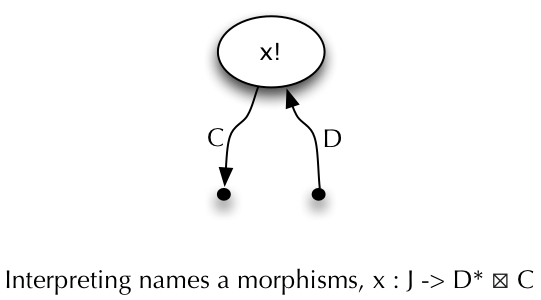
\includegraphics[scale=.50]{images/Pi2HCT-Output.jpg}
%     \caption{ Interpretation of output }
%   \end{center}
% \end{figure}

% \begin{figure}[hbp]
%   \begin{center}
%     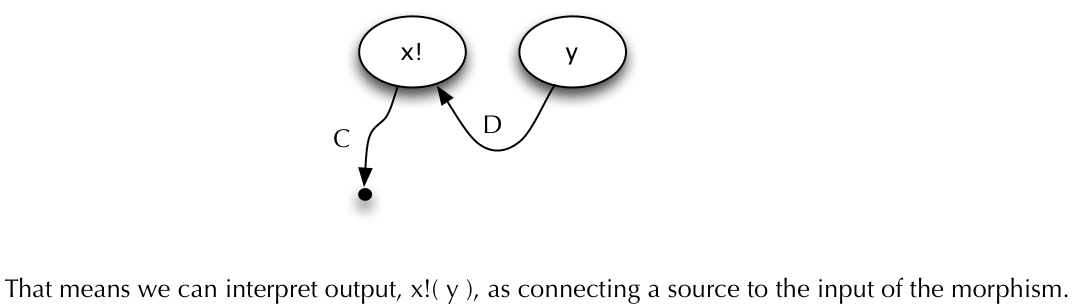
\includegraphics[scale=.50]{images/Pi2HCT-Output2.jpg}
%     \caption{ Interpretation of output - again }
%   \end{center}
% \end{figure}

% \begin{figure}[hbp]
%   \begin{center}
%     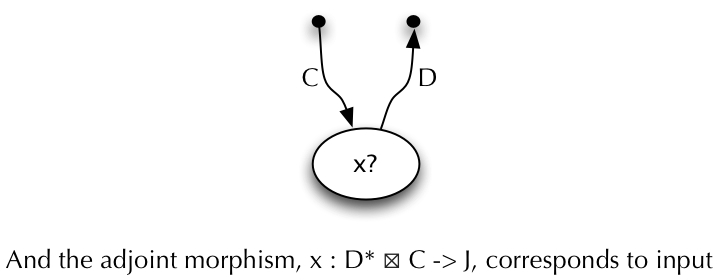
\includegraphics[scale=.50]{images/Pi2HCT-Input.jpg}
%     \caption{ Interpretation of input }
%   \end{center}
% \end{figure}

% \begin{figure}[hbp]
%   \begin{center}
%     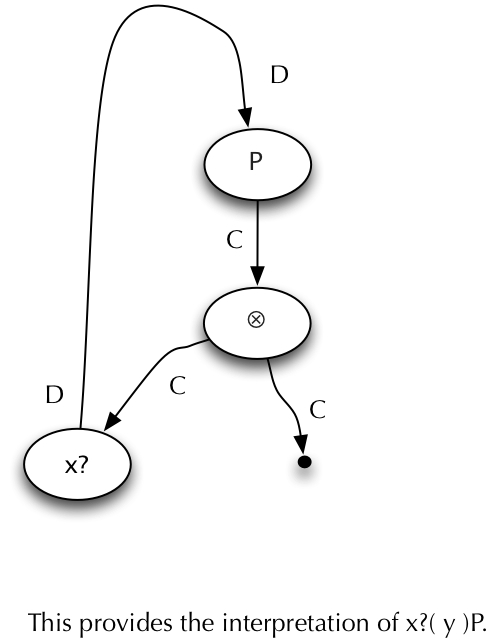
\includegraphics[scale=.50]{images/Pi2HCT-InputGuardedProcess.jpg}
%     \caption{ Interpretation of input guarded process }
%   \end{center}
% \end{figure}

% \begin{figure}[hbp]
%   \begin{center}
%     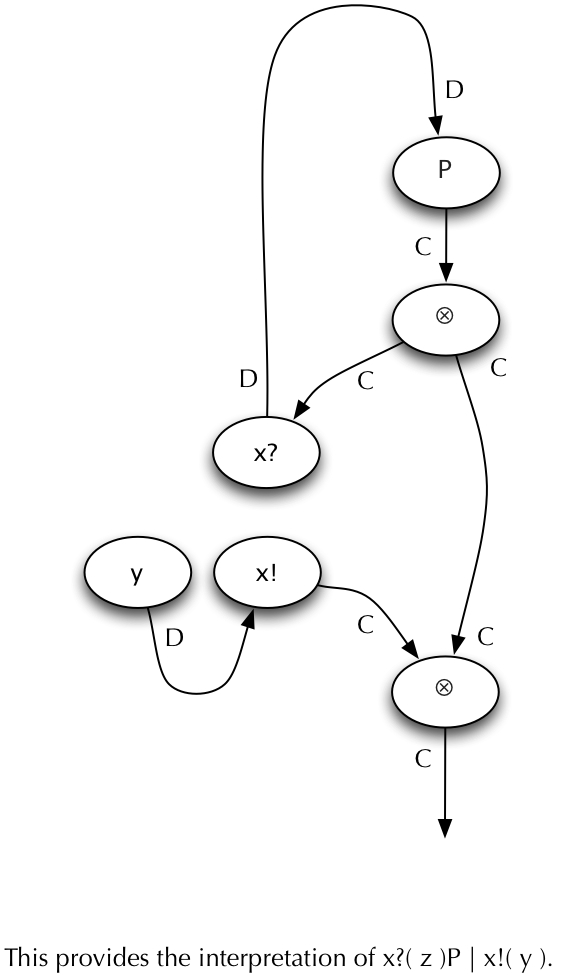
\includegraphics[scale=.50]{images/Pi2HCT-PiRedex.jpg}
%     \caption{ Interpretation of basic {\pic} redex }
%   \end{center}
% \end{figure}

% \begin{figure}[hbp]
%   \begin{center}
%     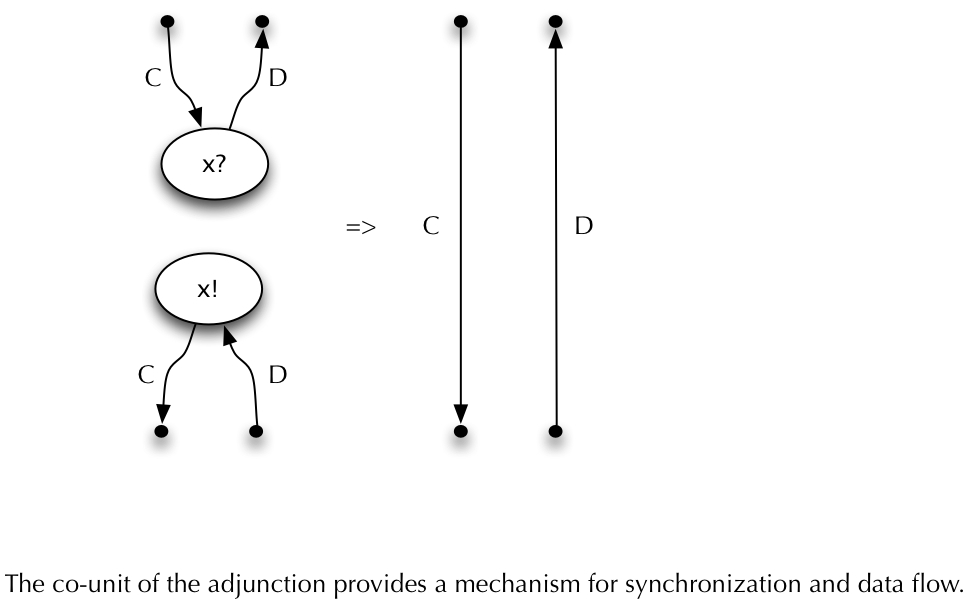
\includegraphics[scale=.50]{images/Pi2HCT-AdjunctionRewriteTemplate.jpg}
%     \caption{ Interpretation of adjunction-based rewrite template }
%   \end{center}
% \end{figure}
\subsection{2-cells}
\label{commdiagram}

\subsection{Semantics}
\begin{equation*}
  \begin{aligned}
    & \meaningof{\pzero} \defneqls \ldots \\
    & \meaningof{{x}{?}{( y_1, \ldots, y_N )} \Rightarrow {P}} \defneqls \ldots \\
    & \meaningof{{x}{!}{( y_1, \ldots, y_N )}} \defneqls \ldots \\
    & \meaningof{\binpar{P}{Q}} \defneqls \ldots \\
  \end{aligned}
\end{equation*}

\section{Conclusions and future work}

TBD \\

\paragraph{Acknowledgments.}
TBD \\

% ------------------------------------------------------------------------
%GATHER{Xbib.bib}   % For Gather Purpose Only
%GATHER{Paper.bbl}  % For Gather Purpose Only
\bibliographystyle{amsplain}
\bibliography{hctm}

% ------------------------------------------------------------------------



% ------------------------------------------------------------------------

\end{document}
% ------------------------------------------------------------------------
